\documentclass{article}
\usepackage{graphicx, amsmath,amssymb,amsthm,fullpage, hyperref, xcolor, subcaption}
\usepackage[numbers,sort&compress]{natbib}
\bibliographystyle{ieee_fullname}
\definecolor{deepblue}{rgb}{0.1, 0.2, 1}
\definecolor{lightred}{rgb}{0.8, 0.05, 0.05}
\hypersetup{
    colorlinks=true,
    urlcolor=deepblue,     % Deep blue for URLs
    pdftitle={cs_486_pre_proposal},
    pdfpagemode=FullScreen,
}
\title{CS 486 Pre-Proposal}
\author{
Safa Obuz \quad Francisco Cruz-Urbanc \quad Krisi Hristova  \\\\
College of Computing and Informatics, Drexel University, Philadelphia, PA, USA \\
{\tt\small \{seo52, fjc59, kh3339\}@drexel.edu}
}

\date{15 April 2025}

\begin{document}

\maketitle

\section*{\textcolor{lightred}{r}Evo\textcolor{lightred}{L}ution: RL for learning optimal agent design}



\paragraph{Overview} Our goal is to create an agent that uses reinforcement learning (RL) to dynamically optimize its physical morphology—such as limb count, joint configuration, and overall shape—to efficiently run. We aim to use Nvidia's \textbf{Isaac Lab} for realistic 3D simulations \cite{orbit}, though it doesn't natively support dynamic morphology adjustments during training.
\paragraph{Proposed Approach} To address this, we plan to pre-select a set of body designs parameterized by URDF files. Each design will be trained separately, evaluated, and iteratively refined by replacing the lowest-performing morphologies. Over successive generations, we expect convergence toward an optimal design. Hence, the name of our approach is inspired by "evolutionary" algorithms.
\paragraph{Backup Plans and Methodology} If the above proves infeasible, we will adopt methods from "Reinforcement Learning for Improving Agent Design" \cite{Ha2018designrl}, using simpler (2D) but more flexible environments such as \textbf{Gymnasium} \cite{gymnasium} and automatic training frameworks like \textbf{Tianshou} \cite{tianshou}. Alternatively, we may leverage \textbf{MuJoCo} \cite{mujoco} for detailed 3D simulations, potentially employing multi-agent RL strategies using \textbf{MARL} \cite{marl}. Additionally, can use \textbf{Weights \& Biases} as a monitoring tool with any of the approaches.
\\\\
We seek feedback on the feasibility and practicality of our proposed solutions, particularly concerning dynamic morphology optimization in the Isaac Lab environment. Please see reference images below \ref{fig:rl-agent} \ref{fig:isaac-sim}.


\section*{Resources}

\href{https://mujoco.readthedocs.io/en/stable/overview.html}{\texttt{https://mujoco.readthedocs.io/en/stable/overview.html}}

\noindent
\href{https://marllib.readthedocs.io/en/latest/}{\texttt{https://marllib.readthedocs.io/en/latest/}}

\noindent
\href{https://github.com/thu-ml/tianshou/tree/master}{\texttt{https://github.com/thu-ml/tianshou/tree/master}}

\noindent
\href{https://gymnasium.farama.org/}{\texttt{https://gymnasium.farama.org/}}

\noindent
\href{https://designrl.github.io/}{\texttt{https://designrl.github.io/}}

\noindent
\href{https://isaac-sim.github.io/IsaacLab/main/index.html}{\texttt{https://isaac-sim.github.io/IsaacLab/main/index.html}}

\noindent
\href{https://github.com/wandb/wandb}{\texttt{https://github.com/wandb/wandb}}

\bibliography{bibliography}
\vspace{0.25in}
\begin{figure}[htbp]
  \centering
  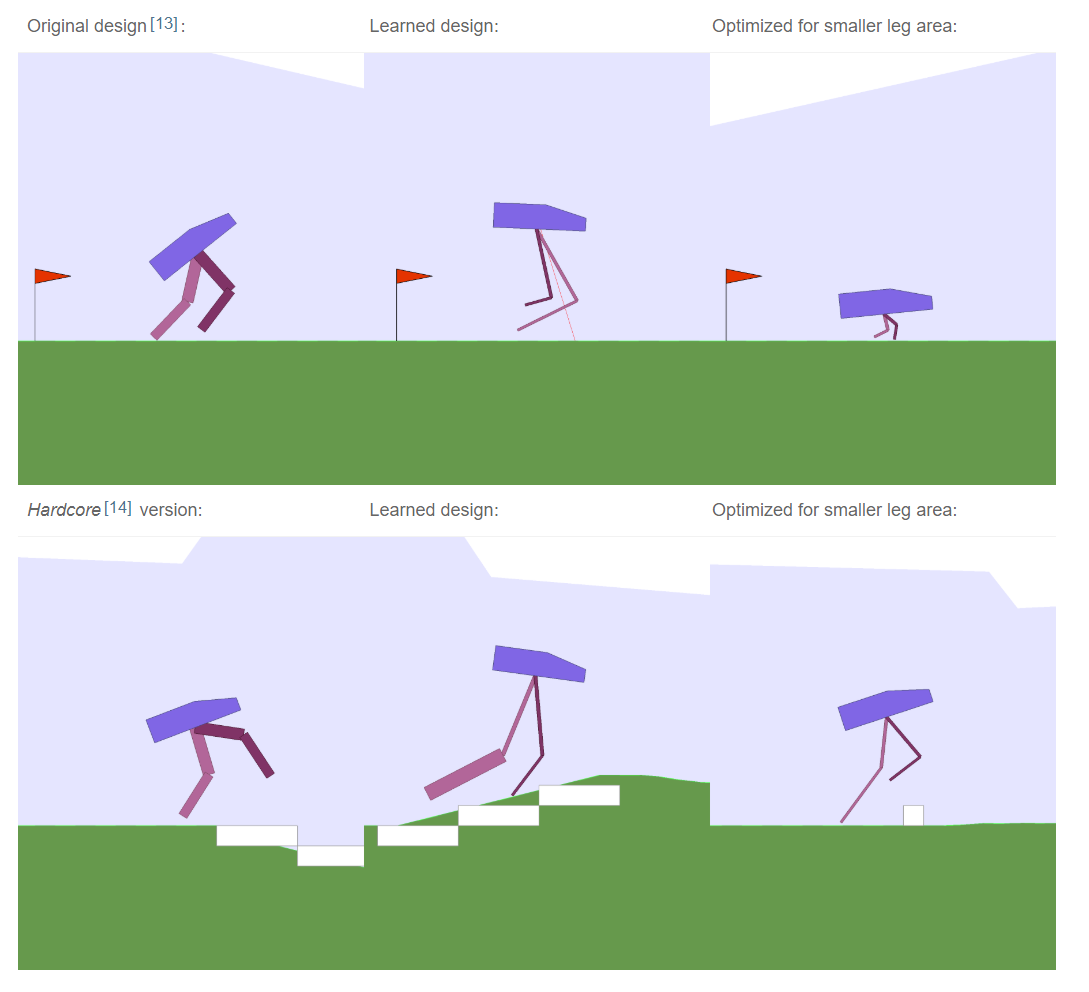
\includegraphics[width=0.4\linewidth]{figures/biped.png}  % adjust path and size
  \caption{An example of an RL agent learning optimal morphology from "Reinforcement Learning for Improving Agent Design”}
  \label{fig:rl-agent}
\end{figure}

\begin{figure}[htbp]
\centering
\begin{subfigure}{0.48\columnwidth}
  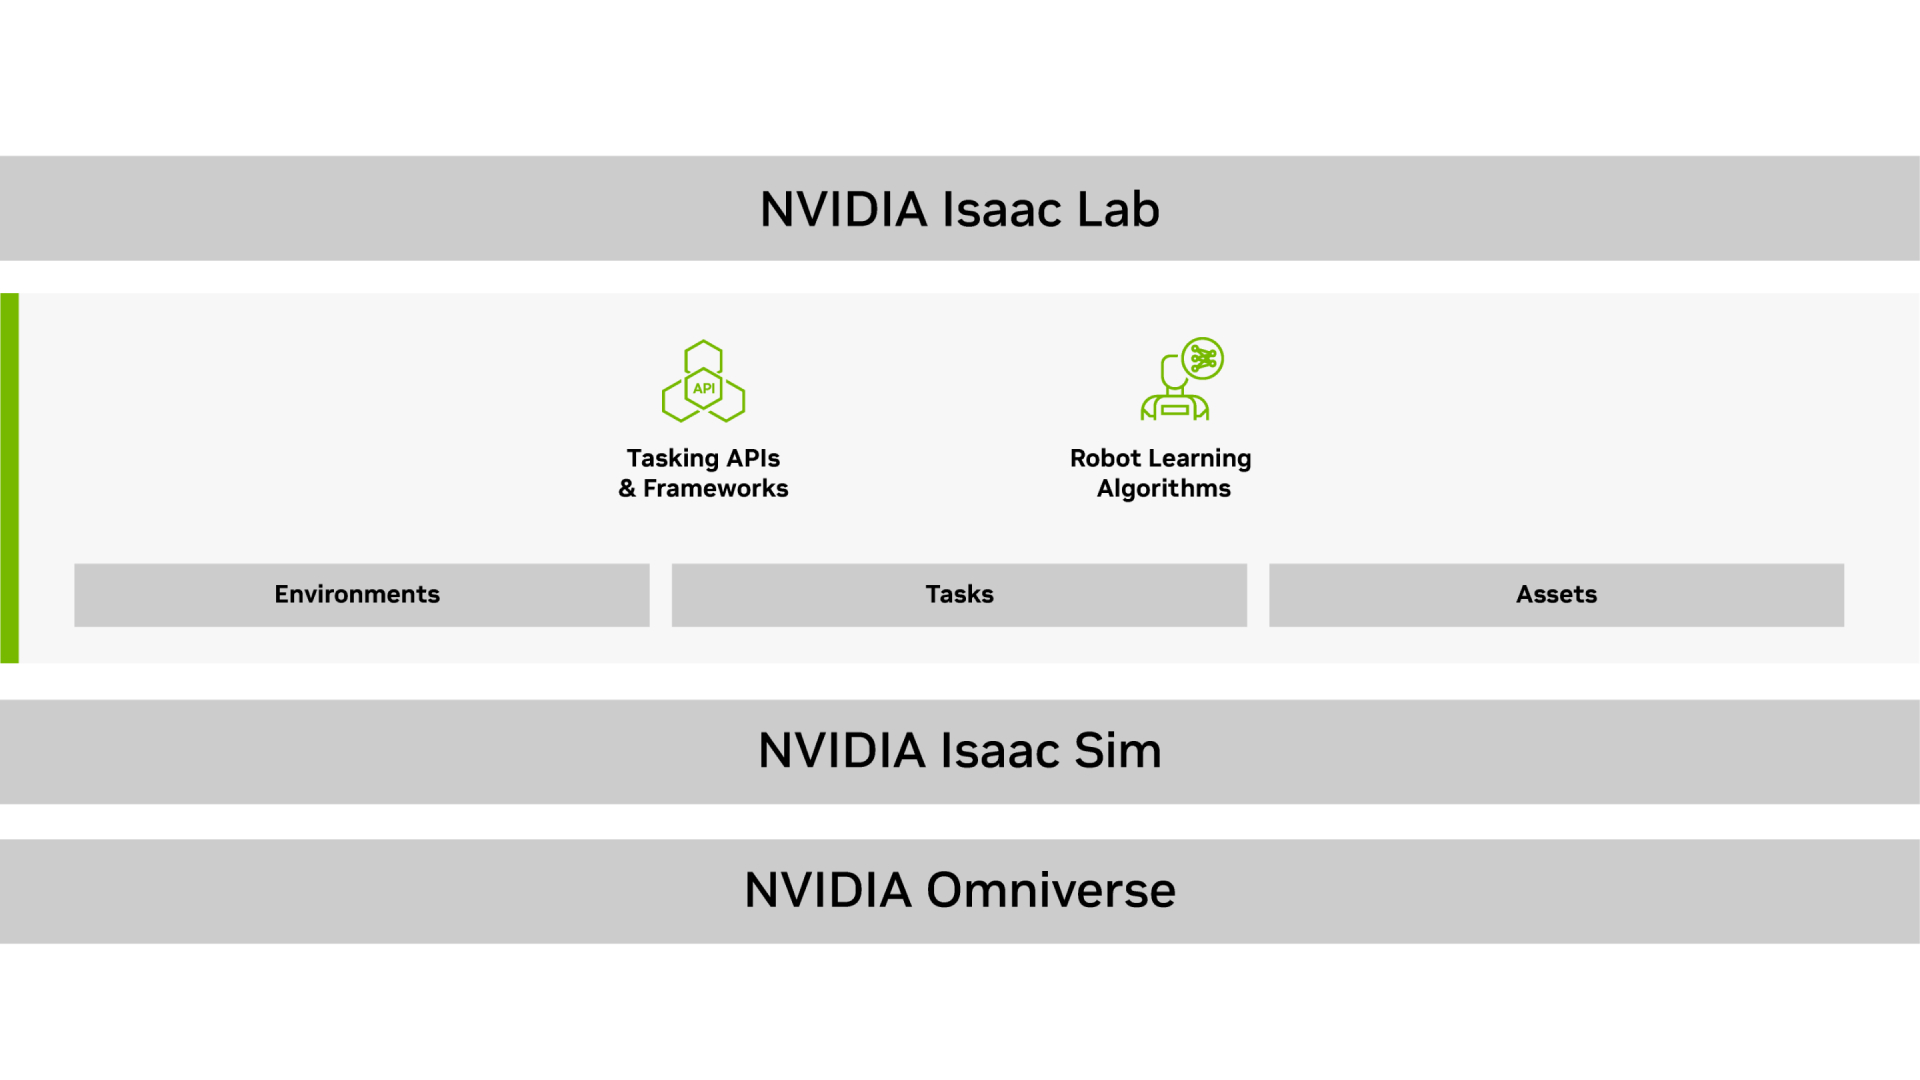
\includegraphics[width=\linewidth]{figures/isaac_lab_stack.jpg}
  \caption*{Nvidia Isaac Simulation Stack}
\end{subfigure}
\hfill
\begin{subfigure}{0.48\columnwidth}
  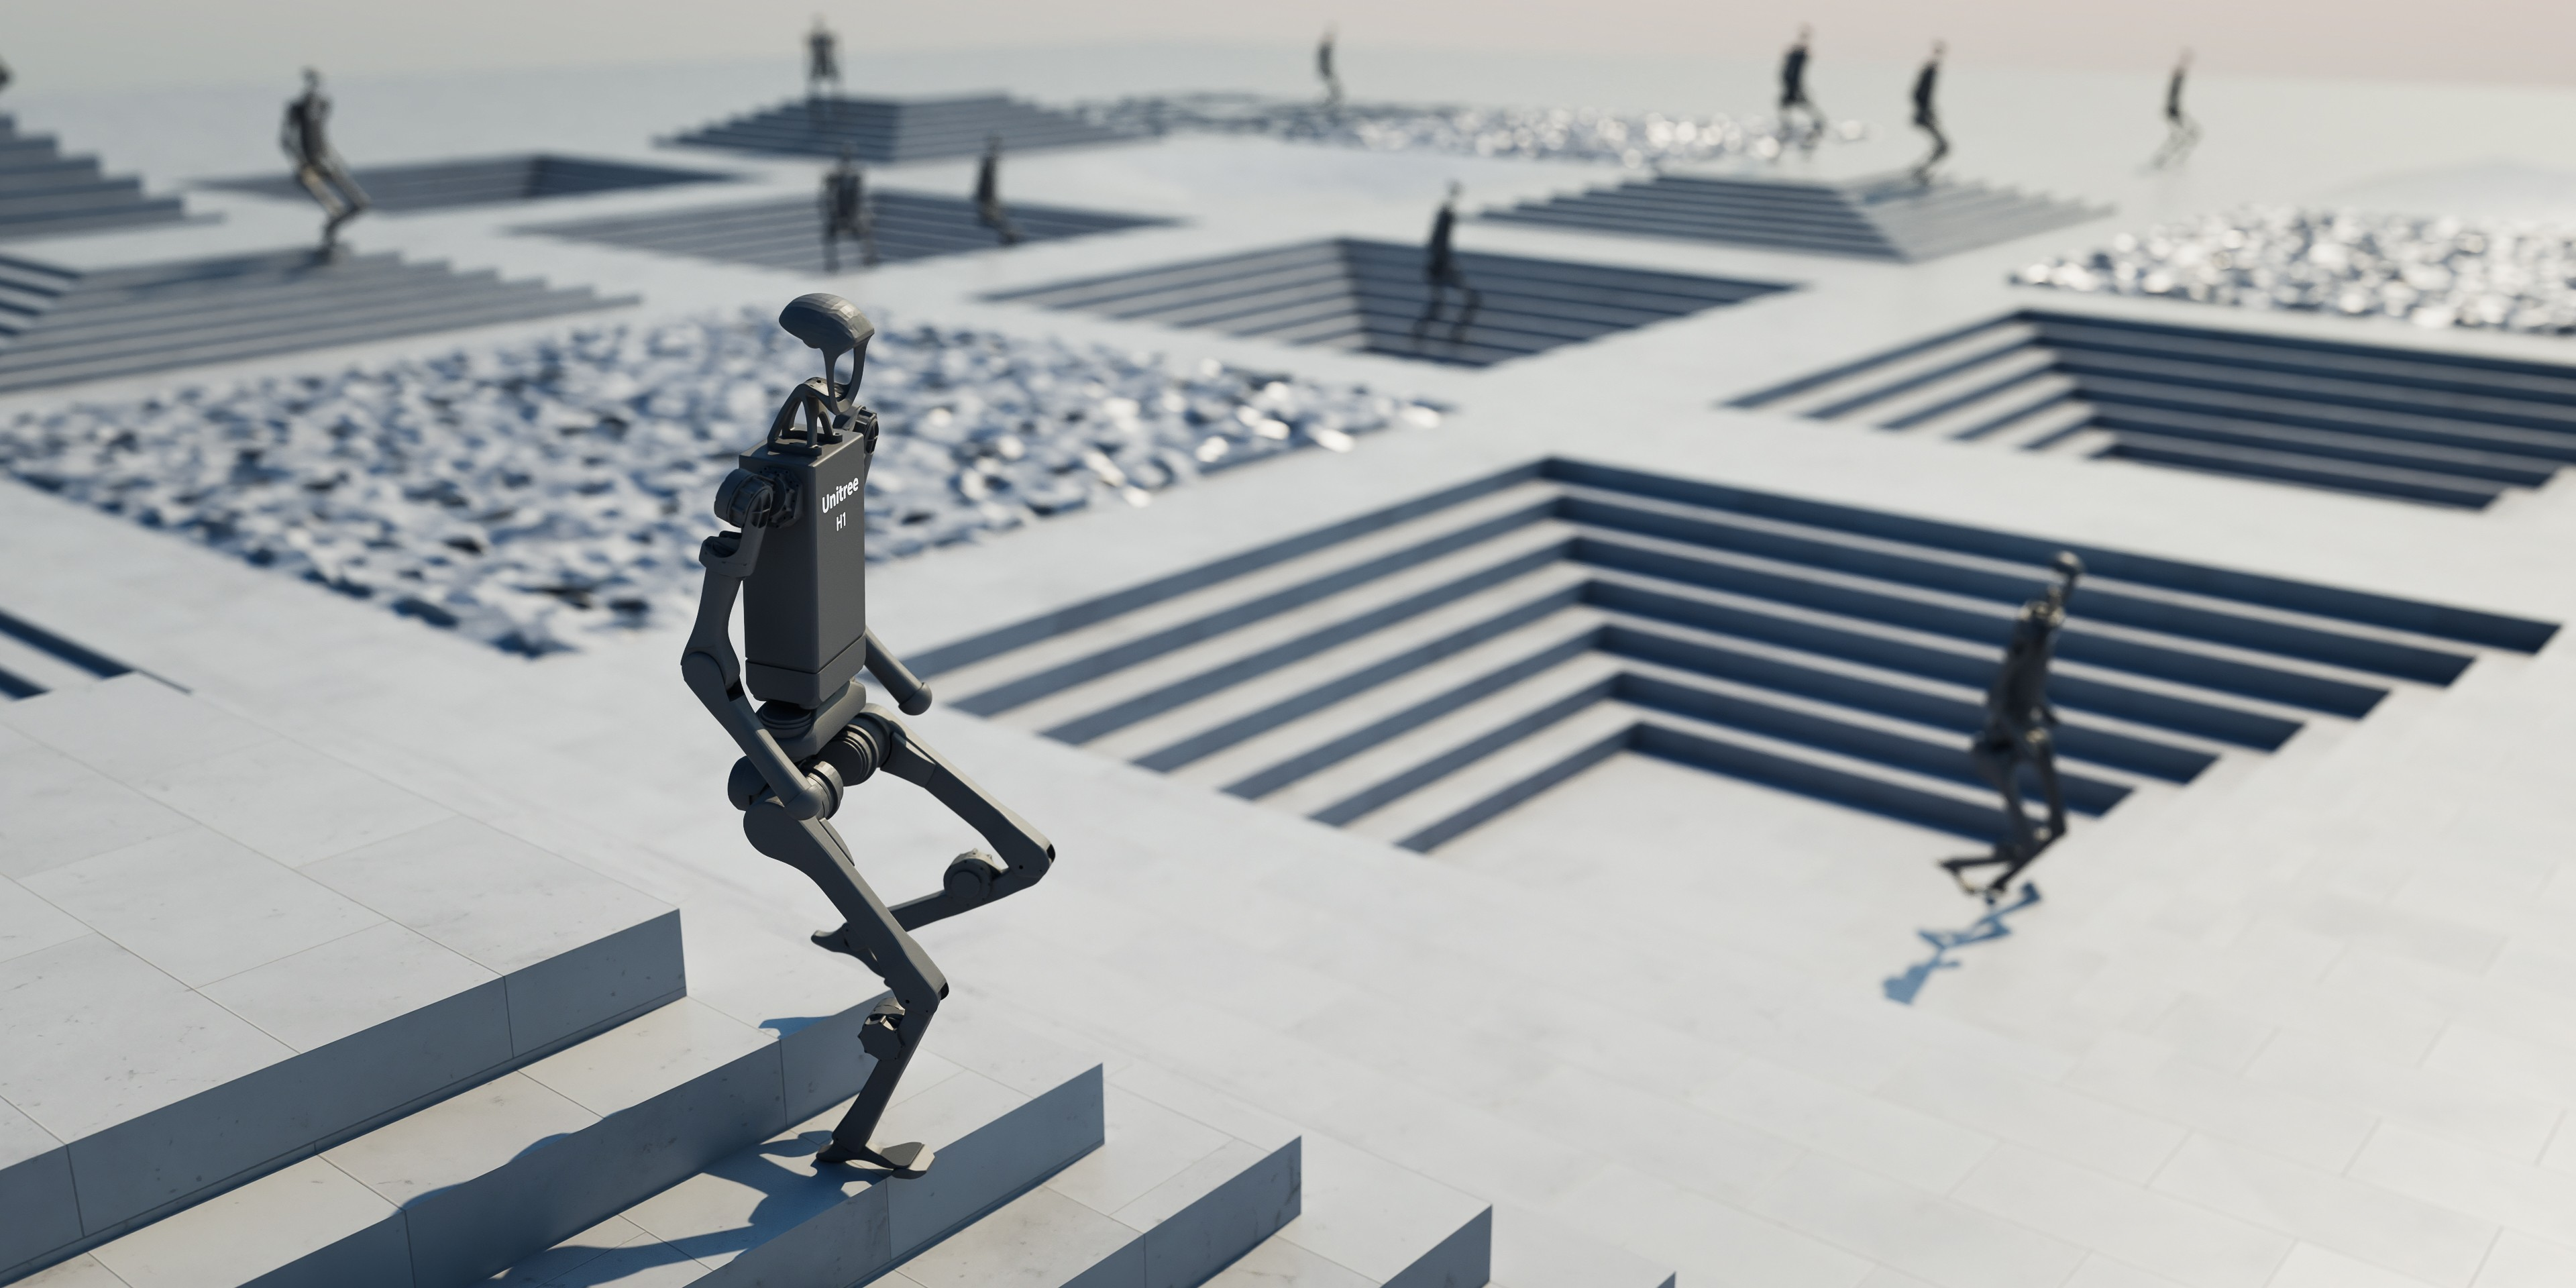
\includegraphics[width=\linewidth]{figures/isaac_lab.jpg}
  \caption*{Rendered simulation environment in Isaac Lab}
\end{subfigure}
\caption{Our preferred RL simulation environment, Isaac Lab}
\label{fig:isaac-sim}
\end{figure}



\end{document}
